\documentclass[twocolumn]{el-author}

%\usepackage[...]{...}      This has been commented out as we are not using any additional packages here.  On the whole, they should be unnecessary.
\newcommand{\hH}{\hat{H}}
\newcommand{\D}{^\dagger}
\newcommand{\ua}{\uparrow}
\newcommand{\nc}{\newcommand}
\nc{\da}{\downarrow} \nc{\hc}{\hat{c}} \nc{\hS}{\hat{S}}
\nc{\bra}{\langle} \nc{\ket}{\rangle} \nc{\eq}{equation (\ref}
\nc{\h}{\hat} \nc{\hT}{\h{T}}\nc{\be}{\begin{eqnarray}}
\nc{\ee}{\end{eqnarray}}\nc{\rd}{\textrm{d}}\nc{\e}{eqnarray}\nc{\hR}{\hat{R}}\nc{\Tr}{\mathrm{Tr}}
\nc{\tS}{\tilde{S}}\nc{\tr}{\mathrm{tr}}\nc{\8}{\infty}\nc{\lgs}{\bra\ua,\phi|}\nc{\rgs}{|\ua,\phi\ket}
\nc{\hU}{\hat{U}}\nc{\lfs}{\bra\phi|}\nc{\rfs}{|\phi\ket}\nc{\hZ}{\hat{Z}}\nc{\hd}{\hat{d}}\nc{\mD}{\mathcal{D}}
\nc{\bd}{\bar{d}}\nc{\bc}{\bar{c}}\nc{\mc}{\mathcal}\nc{\ea}{eqnarray}\nc{\mG}{\mathcal{G}}\nc{\bce}{\begin{center}}
\nc{\ece}{\end{center}}
\date{25th December 2017}

\usepackage{color}
\usepackage{ascmac}
\usepackage{amsmath}
\usepackage{graphicx}
\graphicspath{{./Figure/}}

\begin{document}

\title{Performance of all-optical AND gate using photonic-crystal QDSOA at 160 Gb/s}

\author{T. Matsumoto, G. Hosoya and H. Yashima}

% TODO:�K�؂ȕ\���ɕς���
\abstract{An all-optical AND gate using photonic-crystal quantum dot semiconductor optical amplifiers is designed and its performance is evaluated. The input-output characteristics of the gate are simulated using rate equation model and it is found that the gate can achieve a maximum of approximately 9-dB extinction ratio at 160 Gb/s . The proposed gate is compared with quantum dot semiconductor optical amplifiers AND gate to evaluate its effectiveness with regard to signal output, device size, and power consumption.}

\maketitle

\section{Introduction}
Owing to progressing technology, high-speed and large-capacity data transmission is required to cope with increasing network traffic {\cite{qdsoa_ethernet}}. In current optical networks, an optical signal travels to its destination through optical fibers, and the signal is affected by noise along the way. Thus, re-amplification, re-timing, and re-shaping of the signal are essential for a reliable optical network operation. Currently, electronic components are used to implement these operations. However, these components have low processing speed and consume high energy during optical-to-electrical signal conversion {\cite{3r_regeneration}}. Signal processing equipment that uses all-optical components can avoid these limitations, and researchers are actively pursuing all-optical signal processing components.
Quantum dot semiconductor optical amplifiers (QDSOAs) are optical devices that can be useful in many applications owing to its relatively fast gain recovery time and nonlinear optics {\cite{qdsoa_aosp}}. The confinement of electrons and electron holes in QDs enables fast gain recovery, and gain saturation in the SOA leads to the nonlinear optics.
In contrast, PC is a dielectric material with a periodic pattern of two different refractive indexes, therefore, light waves of a single bandwidth cannot propagate through photonic-crystal (PC). PC waveguide (PCW) exploits this characteristic with a line defect in a PC slab. This defect confines the light waves in the directions perpendicular and parallel to the direction of propagation. Moreover, the dispersion relation between the PC refractive indices can decelerate the wave velocity, which can be useful in cases wherein a PCW is combined with an SOA or QDSOA. \par
Similar to electronic logic gates, all-optical logic gates (AOLGs) can manipulate binary inputs. Although many AOLGs have been developed using a variety of optical materials, the length of these AOLGs tends to be larger than that of electrical logic gates since all-optical components must be long enough to operate the signal. For instance, a typical QDSOA is approximately 2-mm long {\cite{qdsoa_nssm}}, whereas the equivalent transistor used in commercially available electronic devices is approximately 14-nm long {\cite{current_cpu}}. This is an important concerning of the development of devices with high-density integration and minimal energy consumption. Meanwhile, AND gates is one of the most commonly used logic gate. To our knowledge, no research has been conducted on the simulation of a PC-QDSOA all-optical AND gate yet. \par
In this paper, an all-optical AND gate using PC-QDSOA components is proposed.  To demonstrate the effectiveness of the proposed gate, we simulated its input-output characteristics using rate-equation model. Our results indicate that an all-optical AND gate with the PC-QDSOA waveguide could feasibly operate at 160 Gb/s and can achieve a maximum of approximately 9-dB extinction ratio (ER). In addition, substantially low-current injection is required when using the proposed all-optical AND gate.

\section{PC-QDSOA model}
Fig. {\ref{fig:pcqdsoa}} shows schematic design of a PC-QDSOA waveguide. The PC-QDSOAs used in this study comprise GaAs, ${\rm{In_{0.15}Ga_{0.85}As}}$, and InAs at the active region to enhance the optical power whose wavelength is nearby approximately ${\rm{1.3 \mu m}}$ {\cite{theory_of_qdsoa}}. Population inversion in the active regions of the amplifiers is achieved by passing current through laterally doped ${\rm{p^{+}-p-n^{+}}}$ structures. The W1 PCW of the PC-QDSOA allows slow light to be achieved with zero group-velocity and zero third-order dispersions at a specific bandwidth. The W1 PCW is fabricated by creating a line defect in a PC slab, and the slab is fabricated by creating periodic round vacancies on n- and p- clad regions {\cite{how_to_create_pcw}}.

\begin{figure}[htbp]
\begin{center}
  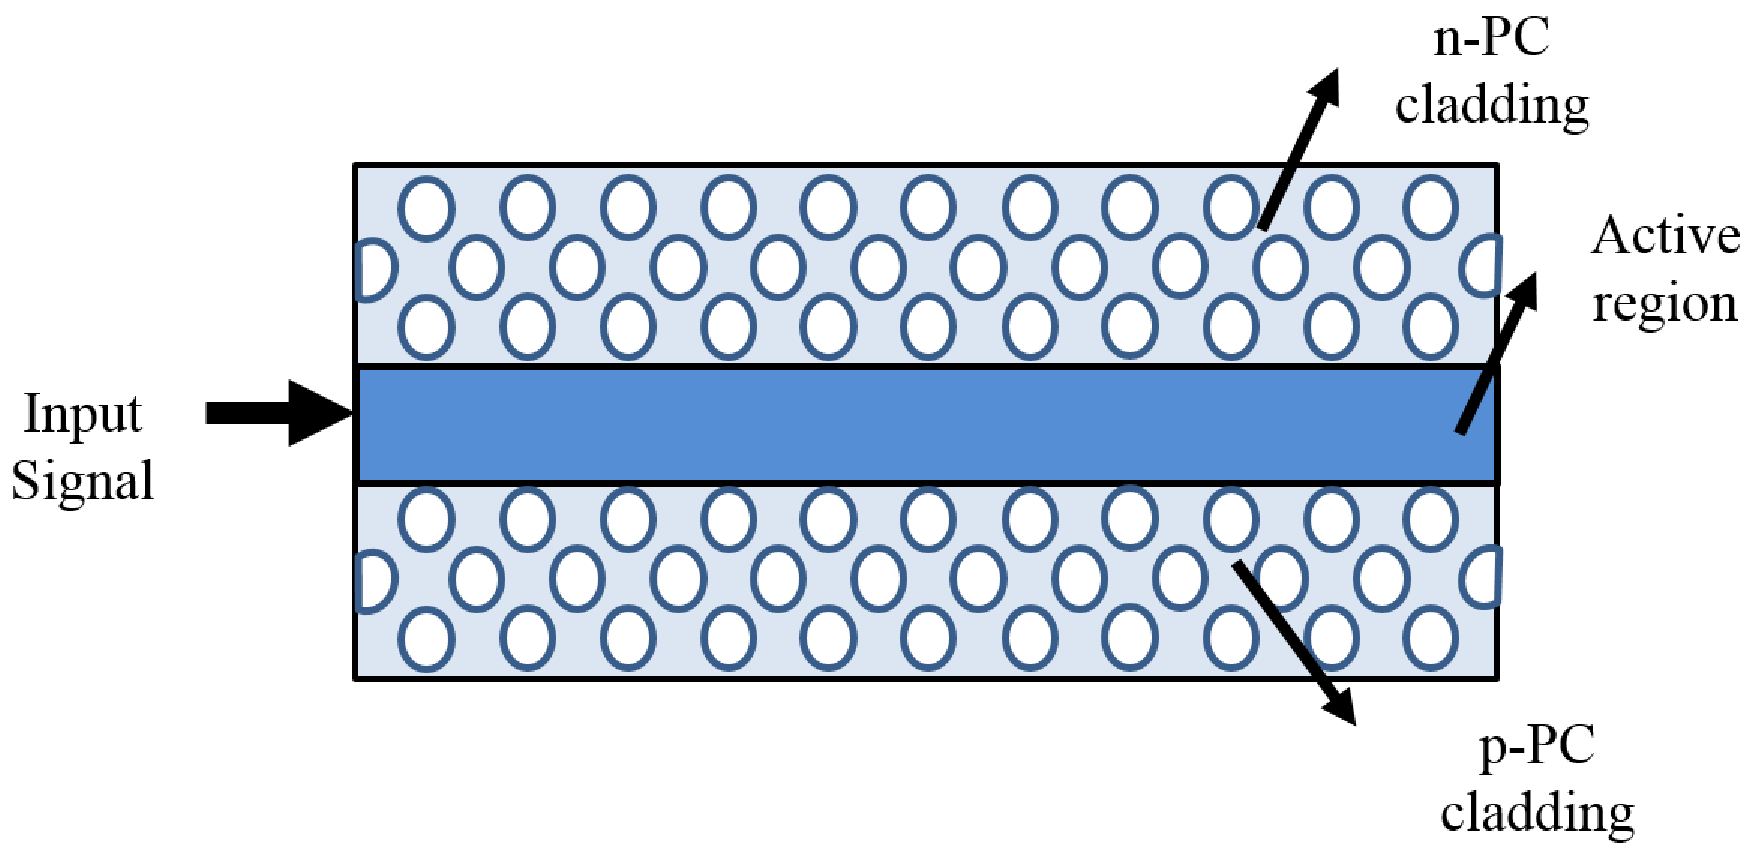
\includegraphics[width=90mm,bb=0 0 1175 568]{pcqdsoa.pdf}
  \caption{Schematic design of the PC-QDSOA waveguide}
  \label{fig:pcqdsoa}
\end{center}
\end{figure}
The operation of the PC-QDSOAs can be studied theoretically using the rate-equation model {\cite{pcqdsoa}}. InAs QDs comprise a ground state (GS), an excited state (ES), and an upper state (US). Quantum wells (QWs) are the common carrier reservoirs in QDs. QDs exhibit homogeneously broadened sizes and shapes, therefore, it is assumed that these states have 2M+1 variables. Thus, the rate equation for the PC-QDSOA is as follows:

\begingroup\makeatletter\def\f@size{7}\check@mathfonts
\begin{eqnarray}
  \label{eq:pc_qd_qw}
  \frac{ {\partial}f^{c(v)}_{w} }{ {\partial}t } & = & 
	\frac{\eta_{inj}I}{qN^{c(v)}_{W}} - 
	\frac{ \sqrt{ f^{c}_{w} f^{v}_{w} } }{ \hat{\tau}^{c(v)}_{wr} } + 
	\frac{ D^{c(v)}_{u} }{ D^{c(v)}_{w} } \sum_{j=1}^{2M+1} G^{c(v)}_{j} \nonumber\\ &&
	\times
	\left(
		\frac{ f^{c(v)}_{u,j} }{ \hat{\tau}^{c(v)}_{uw,j} }	\left(1 - f^{c(v)}_{w} \right) -
		\frac{ f^{c(v)}_{w}  }{ \hat{\tau}^{c(v)}_{wu}  } 	\left(1 - f^{c(v)}_{u,j}\right)
	\right)
  \\
  \label{eq:pc_qd_us}
  \frac{ {\partial}f^{c(v)}_{u,j} }{ {\partial}t } & = & 
	\frac{ f^{c(v)}_{w}  }{ \hat{\tau}^{c(v)}_{wu}  }	\left(1 - f^{c(v)}_{u,j}\right) -
	\frac{ f^{c(v)}_{u,j} }{ \hat{\tau}^{c(v)}_{uw,j} }	\left(1 - f^{c(v)}_{w} \right) + \frac{ D^{c(v)}_{e} }{ D^{c(v)}_{u} } \nonumber\\ &&
	\times \left(
		\frac{ f^{c(v)}_{e,j} }{ \hat{\tau}^{c(v)}_{eu} } \left(1 - f^{c(v)}_{u,j}\right) -
		\frac{ f^{c(v)}_{u,j} }{ \hat{\tau}^{c(v)}_{ue} } \left(1 - f^{c(v)}_{e,j}\right)
	\right)  \nonumber\\ &&
	+ \frac{ D^{c(v)}_{g} }{ D^{c(v)}_{u} } \left(
		\frac{ f^{c(v)}_{g,j} }{ \hat{\tau}^{c(v)}_{gu} } \left(1 - f^{c(v)}_{u,j}\right) -
		\frac{ f^{c(v)}_{u,j} }{ \hat{\tau}^{c(v)}_{ug} } \left(1 - f^{c(v)}_{g,j}\right)
	\right)  \nonumber\\ &&
	- \frac{ \sqrt{ f^{c}_{u,j} f^{v}_{u,j} } }{ \hat{\tau}^{c(v)}_{ur} }
  \\
  \label{eq:pc_qd_es}
  \frac{ {\partial}f^{c(v)}_{e,j} }{ {\partial}t } & = & 
	\frac{ f^{c(v)}_{u,j} }{ \hat{\tau}^{c(v)}_{ue} }	\left(1 - f^{c(v)}_{e,j}\right) -
	\frac{ f^{c(v)}_{e,j} }{ \hat{\tau}^{c(v)}_{eu} }	\left(1 - f^{c(v)}_{u,j}\right) \nonumber\\ &&
	+ \frac{ D^{c(v)}_{g} }{ D^{c(v)}_{e} } \left(
		\frac{ f^{c(v)}_{g,j} }{ \hat{\tau}^{c(v)}_{ge} } \left(1 - f^{c(v)}_{e,j}\right) -
		\frac{ f^{c(v)}_{e,j} }{ \hat{\tau}^{c(v)}_{eg} } \left(1 - f^{c(v)}_{g,j}\right)
	\right)  \nonumber\\ &&
	- \frac{ 1 }{ N^{c(v)}_{E,j} } \sum_{k} \frac
		{\Gamma_{k}P_{k,in}g^{e}_{j,k}\left[e^{\left(\left[g_{mod}(t,\lambda_{k}) - \alpha(\lambda_{k})\right]L_{ca}\right)} - 1\right]}
		{\hbar \omega_{k}\left[g_{mod}(t,\lambda_{k}) - \alpha(\lambda_{k})\right]} \nonumber\\ &&
	\times
	\left( f^{c}_{e,j} + f^{v}_{e,j} - 1 \right)
  \\
  \label{eq:pc_qd_gs}
  \frac{ {\partial}f^{c(v)}_{g,j} }{ {\partial}t } & = & 
	\frac{ f^{c(v)}_{u,j} }{ \hat{\tau}^{c(v)}_{ug} }	\left(1 - f^{c(v)}_{g,j}\right) -
	\frac{ f^{c(v)}_{g,j} }{ \hat{\tau}^{c(v)}_{gu} }	\left(1 - f^{c(v)}_{u,j}\right) \nonumber\\ &&
	\frac{ f^{c(v)}_{e,j} }{ \hat{\tau}^{c(v)}_{eg} } \left(1 - f^{c(v)}_{g,j}\right) -
	\frac{ f^{c(v)}_{g,j} }{ \hat{\tau}^{c(v)}_{ge} } \left(1 - f^{c(v)}_{e,j}\right) \nonumber\\ &&
	- \frac{ \sqrt{ f^{c}_{g,j} f^{v}_{g,j} } }{ \hat{\tau}_{dr} } - \frac{1}{N^{c(v)}_{G,j}} \nonumber\\ &&
	\times \left(\sum_{k} 
	\frac
		{\Gamma_{k}P_{k,in}g^{g}_{j,k}\left[e^{\left(\left[g_{mod}(t,\lambda_{k}) - \alpha(\lambda_{k})\right]L_{ca}\right)} - 1\right]}
		{\hbar \omega_{k}\left[g_{mod}(t,\lambda_{k}) - \alpha(\lambda_{k})\right]} + \right. \nonumber\\ && 
	\left.
	\frac
		{\Gamma_{p}P_{p}g^{e}_{j,p}\left[e^{\left(\left[g_{mod}(t,\lambda_{p}) - \alpha(\lambda_{p})\right]L_{ca}\right)} - 1\right]}
		{\hbar \omega_{p}\left[g_{mod}(t,\lambda_{p}) - \alpha(\lambda_{p})\right]}
	\right) \nonumber\\ &&
	\times
	\left( f^{c}_{g,j} + f^{v}_{g,j} - 1 \right)
\end{eqnarray}
\endgroup
where $f^{c(v)}_{w}$ represents the carrier occupancy of the QW. Likewise, $f^{c(v)}_{u,j},f^{c(v)}_{e,j},f^{c(v)}_{g,j}$ represent the carrier occupancy of the $j$th group of US, ES, and GS, respectively. $\Gamma_{k}$ is the optical confinement factor at wavelength $\lambda_{k}$. The power of the $k$th photon mode and probe signal are represented as $P_{k,in}$ and $P_{p}$, respectively. The term $\alpha(\lambda_{(k,p)})$ is the loss coefficient at the wavelength $\lambda_{(k,p)}$, which is the sum of the scattering and absorption losses. The term $g_{mod}(t,\lambda_{(k,p)})$ is the effect on linear modal gain caused by slow light, and it can be expressed as the product of the slowdown factor, optical-confinement factor, and linear material gain of the active region. Similarly,
$g^{g(e)}_{j,k}$ is the linear optical gain that the GS (ES) of the $j$-th QD group provides to the $k$-th photon mode. More details about the PC-QDSOA structure are provided in reference {\cite{pcqdsoa}}.

\section{AND gate model}
Fig. {\ref{fig:and_gate}} schematizes the PC-QDSOA all-optical AND gate. Following the labels in Fig. {\ref{fig:and_gate}}, the operation of AND gate is described as follows: a modulated data signal A (at wavelength $\lambda_{A}$) and a clock signal (at wavelength $\lambda_{C}$) are injected to the PC-QDSOA1. Signal A with high intensity causes carrier depletion which leads to gain saturation. It causes intensity reduction of clock signal in PC-QDSOA1, therefore, the logic output is always NOT A. In the same way as this operation, the modulated data signal NOT A (at wavelength $\lambda_{C}$) and a modulated data signal B (at wavelength $\lambda_{B}$, which can be equal to the wavelength of signal A) are injected to PC-QDSOA2, and the logic output is then A AND B. Though, the structure of some of other all-optical logic gates is based on Mach-Zehnder interferometer {\cite{mzi_gate}} with exploiting cross phase modulation, one of the proposed gate is less complex with exploiting cross gain modulation. Owing to the structural characteristic, the proposed gate allows the PC-QDSOA1 to be different from the PC-QDSOA2 in physical parameters such as device length and quantum dot density.

\begin{figure}[htbp]
\begin{center}
  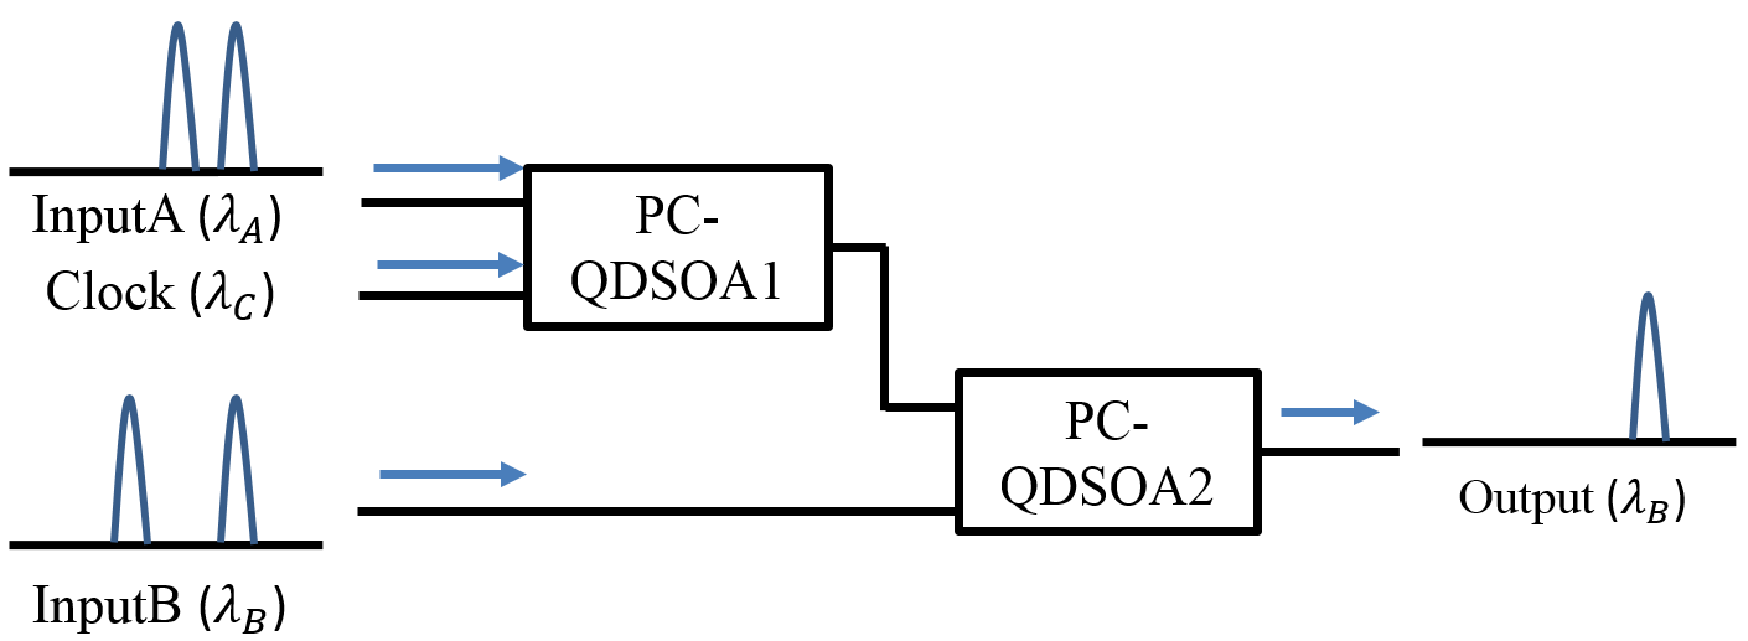
\includegraphics[width=100mm,bb=0 0 1410 517]{and_gate.pdf}
  \caption{Schematic of the PC-QDSOA all-optical AND gate}
  \label{fig:and_gate}
\end{center}
\end{figure}

\section{Results}
The operation of the proposed gate is simulated using MATLAB 2016b and Optisystem 14.0.0. The physical parameters used for solving the rate equation are provided in reference {\cite{pcqdsoa}}. Table. {\ref{tb:param}} lists the fixed parameters used for the simulation in this paper. The pulses are Gaussian shaped. \par
\begin{table}[htbp]
\begin{center}
  \centering
  \caption{Fixed parameters used in simulation}
  \begin{tabular}{|c|c|c|} \hline
    Parameter & Value & Unit \\ \hline
    Maximum power of Input A & 10 & mW \\ \hline
    Maximum power of Input B & 1 & $\mu W$ \\ \hline
    Maximum power of Clock & 100 & $\mu W$ \\ \hline
    Wavelength of Input A & 1307 & nm \\ \hline
    Wavelength of Input B & 1307 & nm \\ \hline
    Wavelength of Clock & 1310 & nm \\ \hline
    Full width at half maximum of pulse & 1.2 & ps \\ \hline
    Transmission speed & 160 & Gb/s \\ \hline
  \end{tabular}
  \label{tb:param}
\end{center}
\end{table}
To evaluate the proposed gate, the eye diagram, ER, and Q-factor are used as metrics. The ER can be represented as $ER[dB] = 10\log_{10} \left(P^{1}_{min} / P^{0}_{max} \right)$. $P^{1}_{min}$ represents minimum power of the binary signal ``1'' and $P^{0}_{max}$ represents the maximum power of the binary signal ``0''. The Q-factor can be represented as $Q = (S_{1}-S_{0})/(\sigma_{1}+\sigma_{0}) ${\cite{q_factor}} where $S_{1}$, and $S_{0}$ are the average powers of binary signals ``1'' and ``0'', and $\sigma_{1}$ and $\sigma_{0}$ are the standard deviations of those signals. In this paper, the large numbers of these metrics represent the proposed gate is more appropriate for an all-optical AND gate. \par
Fig. {\ref{fig:output_signal}} shows the simulation results for the input-output characteristics with 6-mA current injection. Fig. {\ref{fig:eye_dia}} shows an eye diagram of the output signal. The ER and Q-factor for the output signal are 8.58 dB and 7.41, respectively. These results show that the proposed gate can operate as an AND gate at 160 Gb/s {\cite{extinction_ratio}}. \par
\begin{figure}[htbp]
\begin{center}
  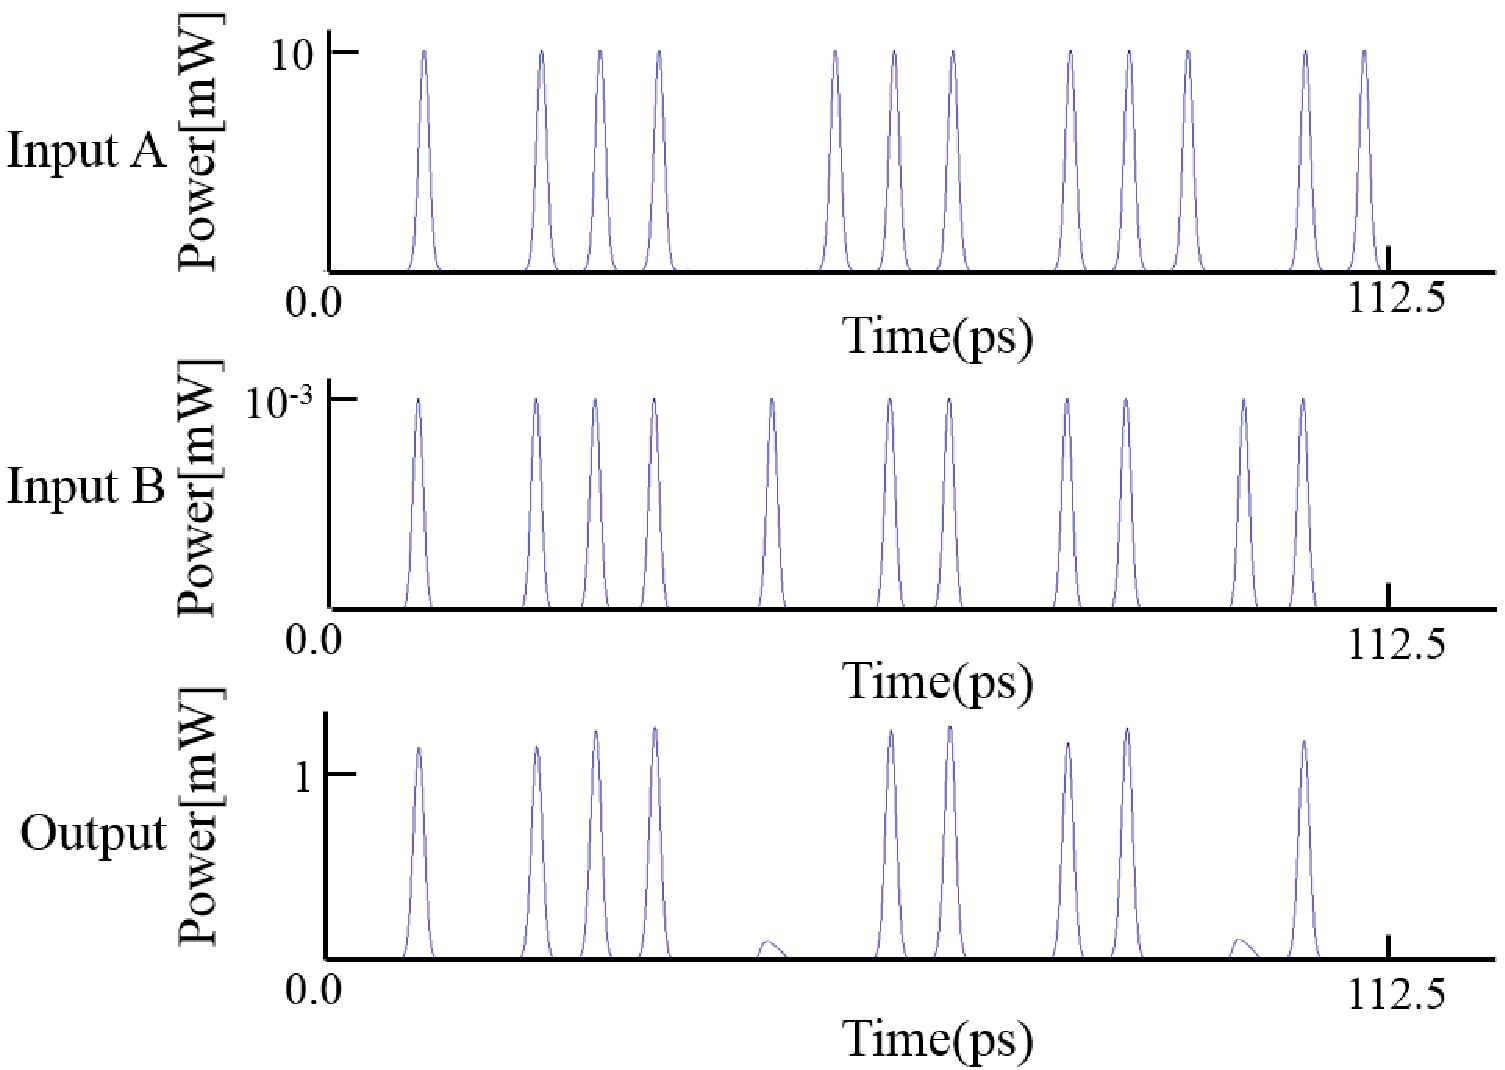
\includegraphics[width=100mm,bb=0 0 963 685]{in-out.pdf}
  \caption{Input-output characteristics for PC-QDSOA all-optical AND gate when current injection is 6 mA}
  \label{fig:output_signal}
  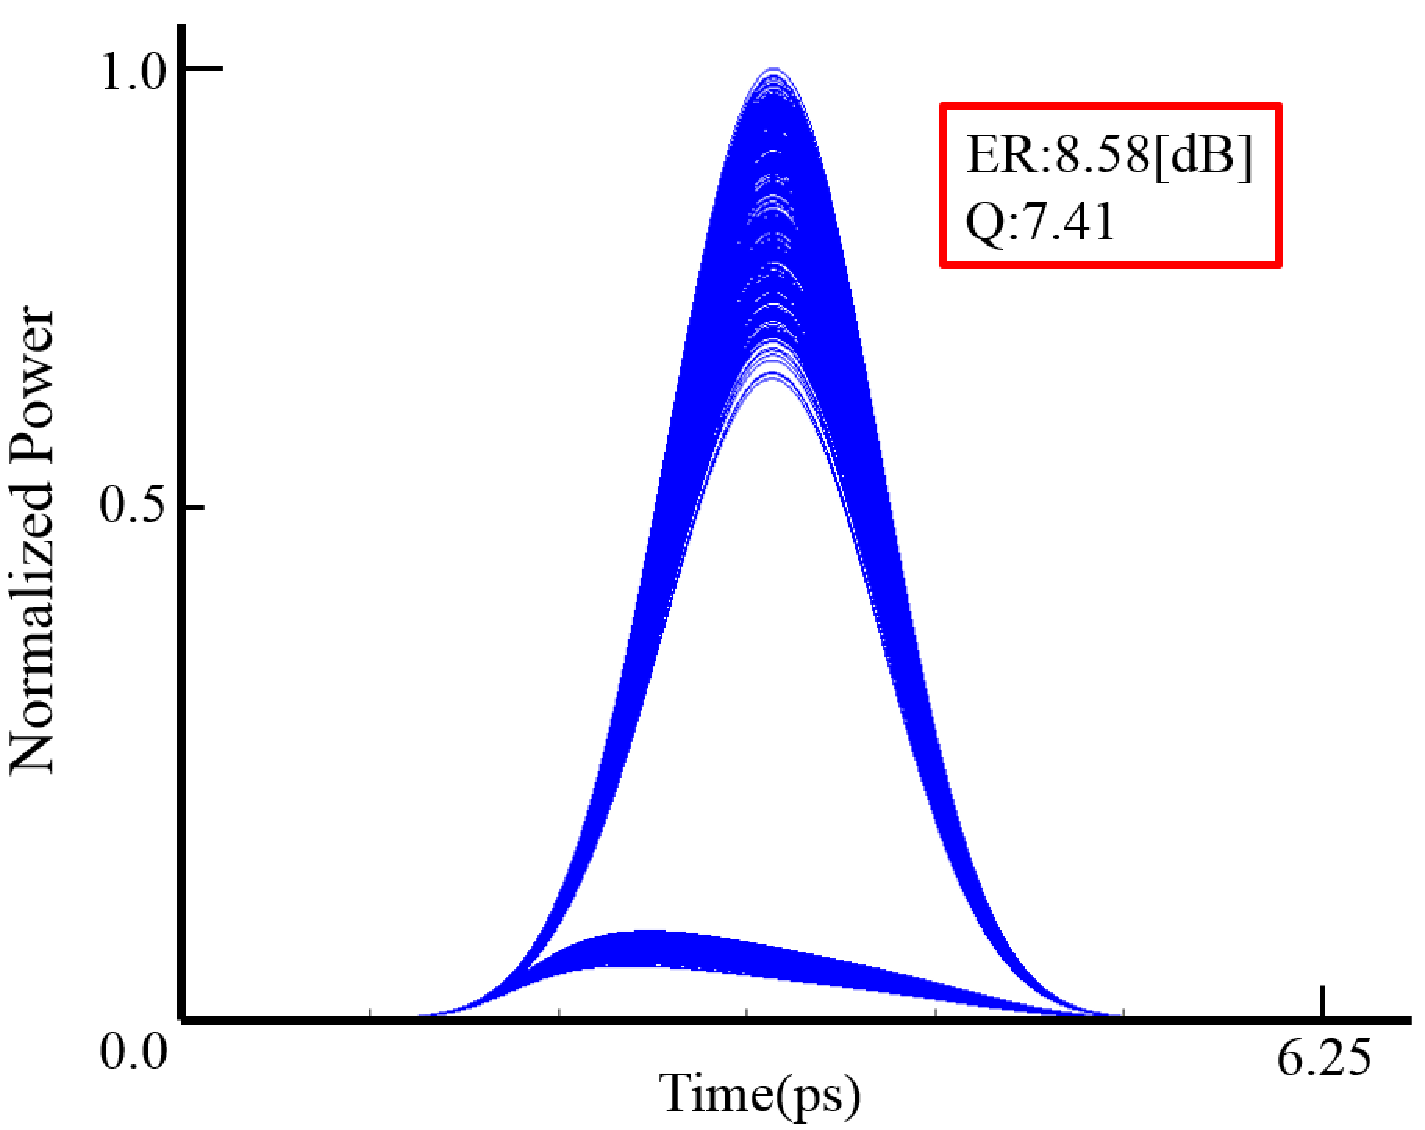
\includegraphics[width=80mm,bb=0 0 912 723]{eyedia_6mA.pdf}
  \caption{Eye diagram of the output signal with 6-mA current injection}
  \label{fig:eye_dia}
\end{center}
\end{figure}
Since the gain recovery time varies with the level of current injection, we also investigate the effect of varying current injection on the power output from the proposed AND gate. Figs. {\ref{fig:pcqdsoa_different_pump_current_ERs}} and {\ref{fig:pcqdsoa_different_pump_current_Qs}} show the ERs and Q-factors of the output signals with different injected currents, respectively. The ERs and Q-factors improve with increasing current injection because pattern effects decrease. When current injection $I \geq$ 9 mA, the ERs change slightly because the maximum gain-recovery time is limited by carrier-relaxation and capture times. 

To quantify the effectiveness of the proposed gate, the performance is compared with those of QDSOA AND gate. Schematic diagram of this gate is same as the proposed design. Physical parameters and the methods used to simulate the QDSOA AND gate are provided in reference {\cite{qdsoa_nssm}}. Figs. {\ref{fig:comp_ERs}} and {\ref{fig:comp_Qs}}, respectively, plot ERs and Q-factors vs. current injection for both QDSOA AND gate and the proposed PC-QDSOA AND gate. To obtain ER of approximately 7.5 dB, the QDSOA AND gate requires 3000-mA injected current, whereas the proposed design requires only 5 mA. Likewise, Fig. {\ref{fig:comp_Qs}} shows that to obtain a Q-factor of approximately 5, the QDSOA AND gate requires 2800-mA injected current, whereas the proposed design requires only 4 mA. Moreover, the QDSOA is 2-mm long, whereas the proposed PC-QDSOA is 125-${\rm{\mu m}}$ long. This comparison demonstrates that the proposed gate reduces energy consumption and device volume compared with QDSOA AND gates.
\begin{figure}[htbp]
\begin{center}
  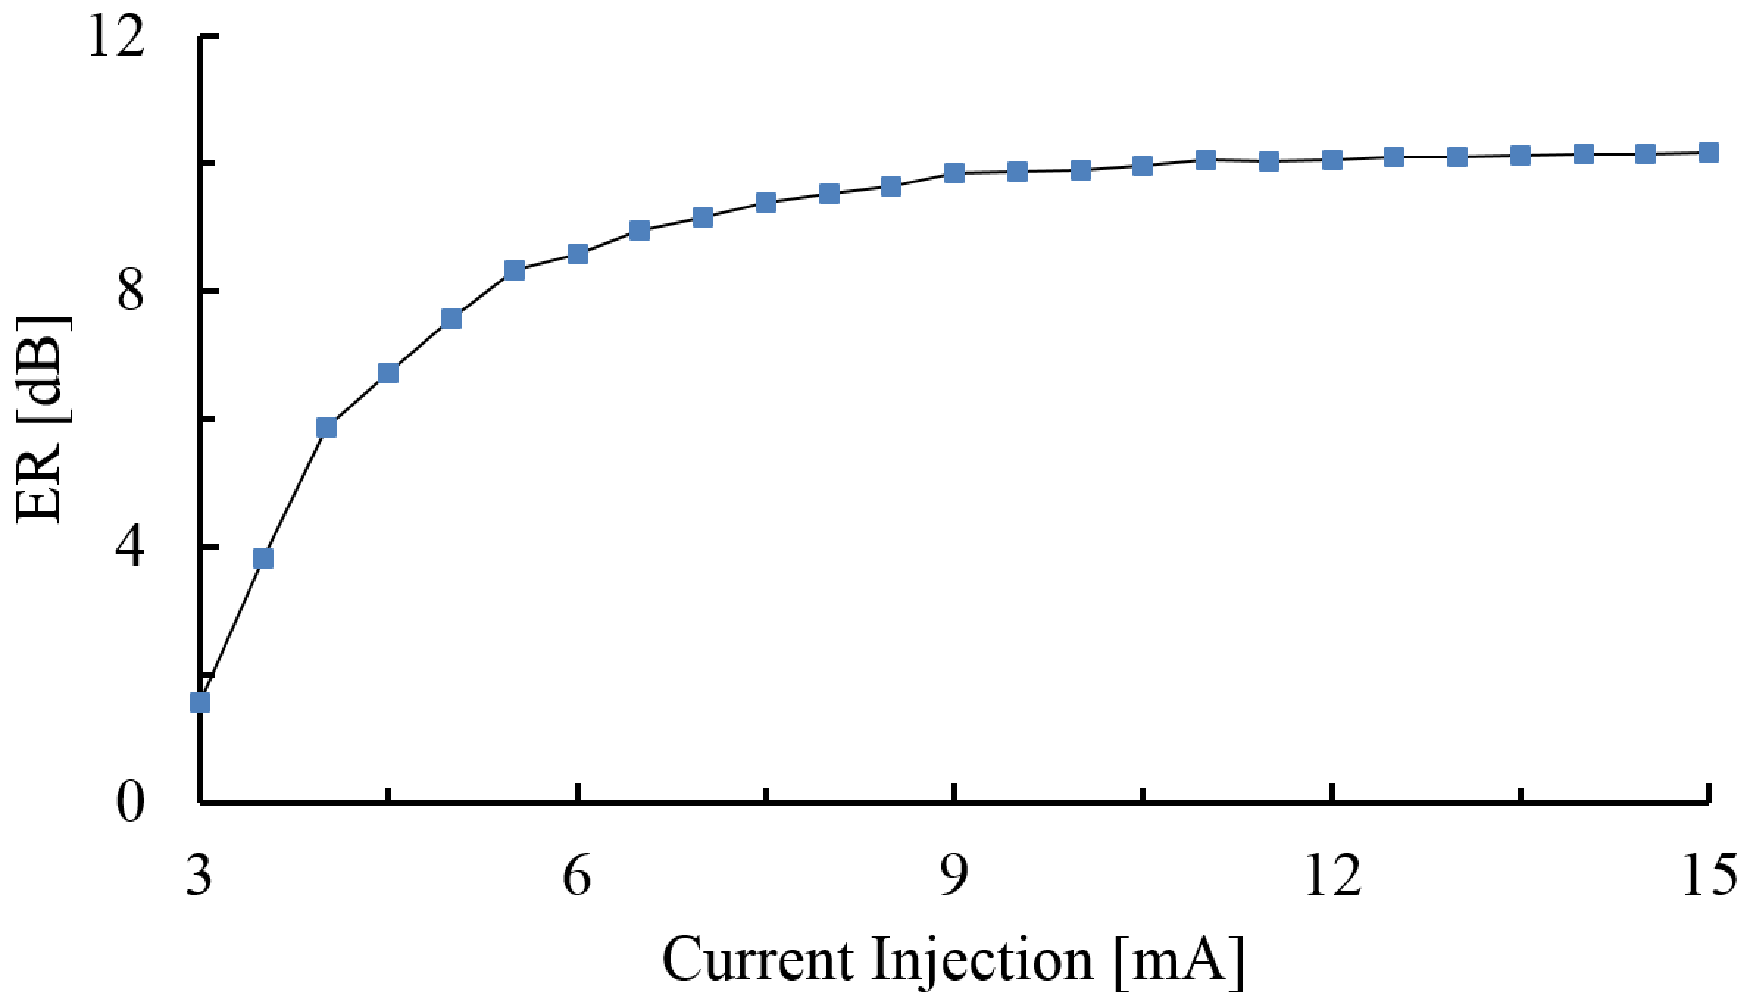
\includegraphics[width=80mm,bb=0 0 1196 685]{pcqdsoa_ERs.pdf}
  \caption{ERs with varying current injection}
  \label{fig:pcqdsoa_different_pump_current_ERs}
  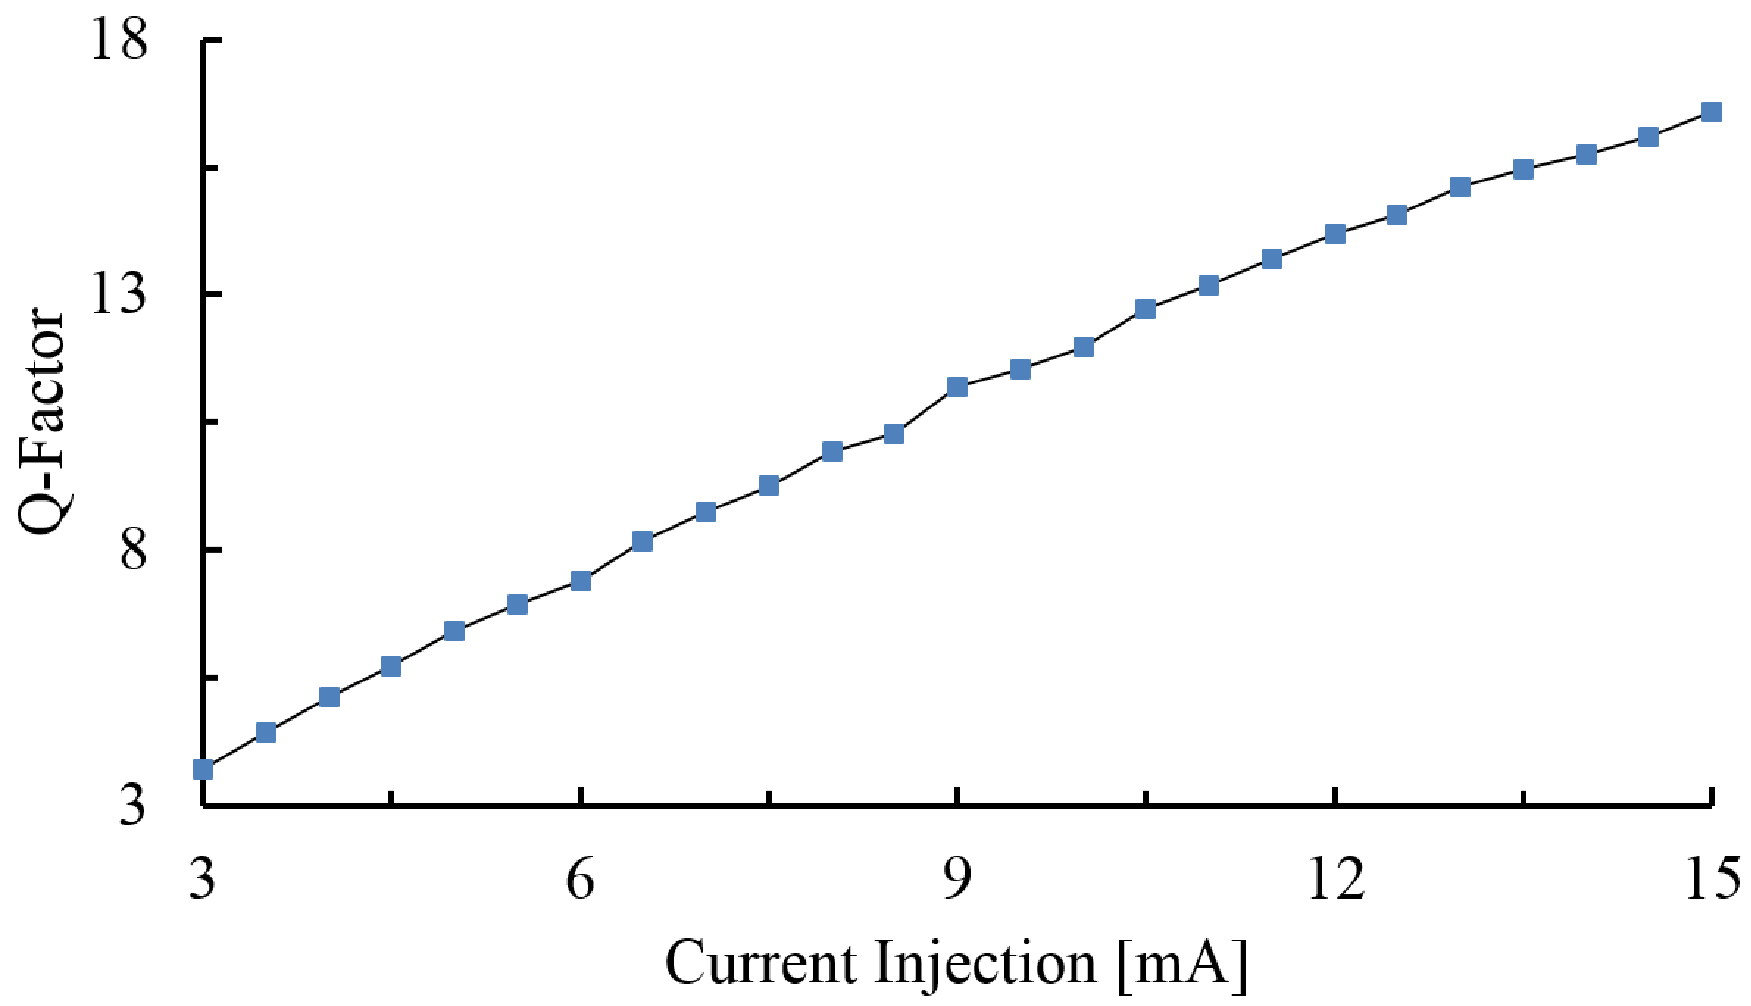
\includegraphics[width=80mm,bb=0 0 1191 684]{pcqdsoa_Qs.pdf}
  \caption{Q-factors with varying current injection}
  \label{fig:pcqdsoa_different_pump_current_Qs}
  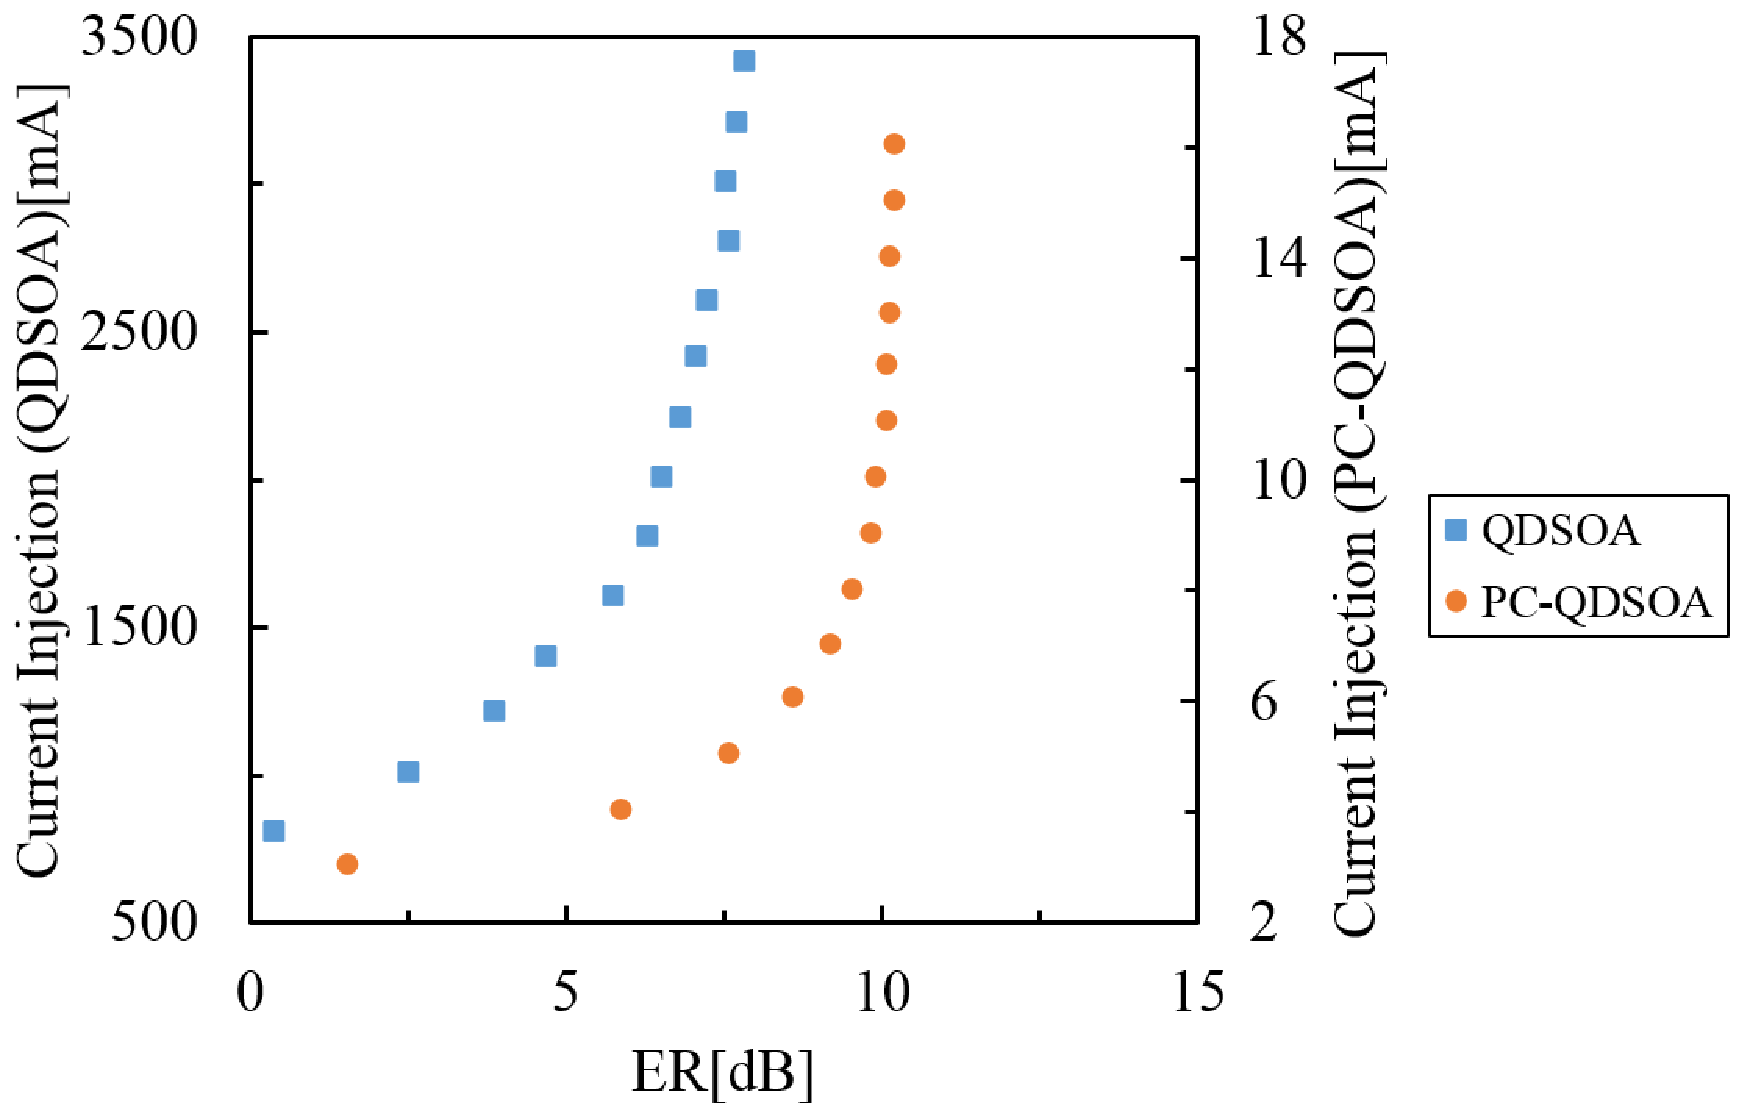
\includegraphics[width=100mm,bb=0 0 1112 709]{qdsoa_vs_pcqdsoa_ERs.pdf}
  \caption{ERs of QDSOA and PC-QDSOA all-optical AND gate with varying current injection}
  \label{fig:comp_ERs}
  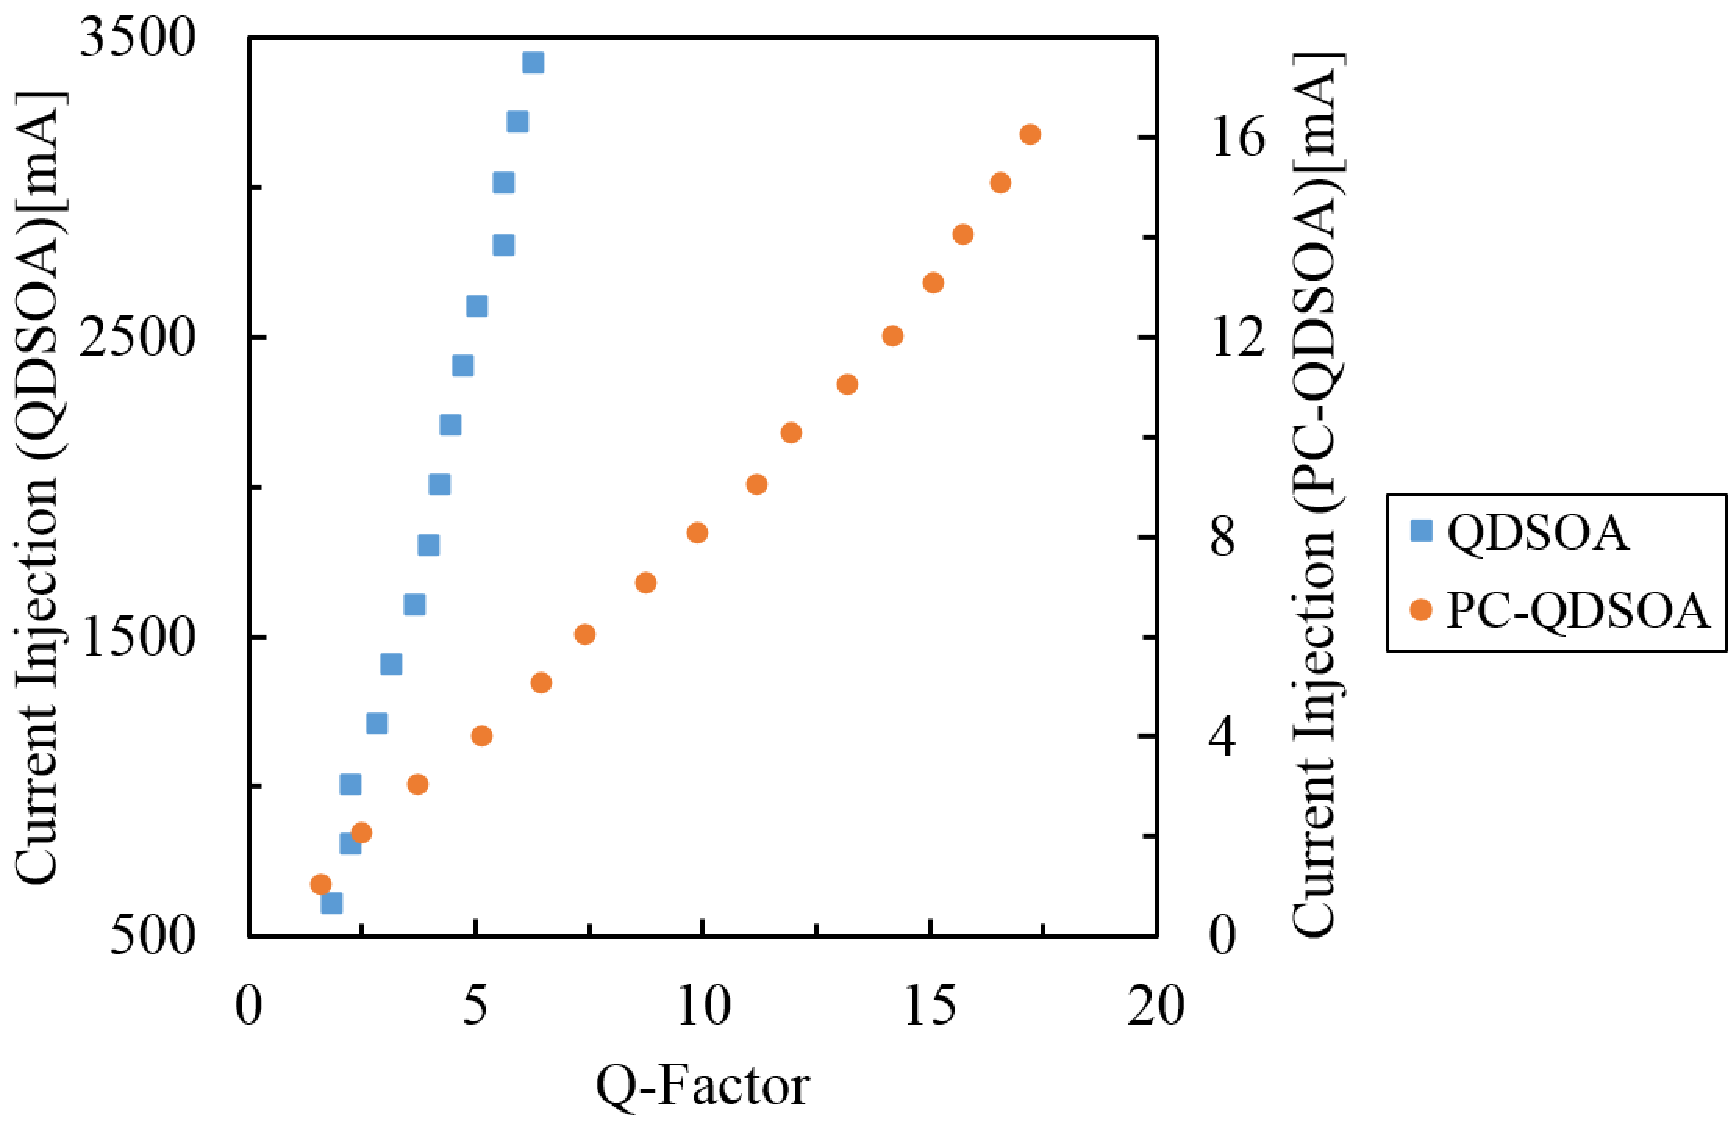
\includegraphics[width=100mm,bb=0 0 1110 719]{qdsoa_vs_pcqdsoa_Qs.pdf}
  \caption{Q-factors of QDSOA and PC-QDSOA all-optical AND gate with varying current injection}
  \label{fig:comp_Qs}
\end{center}
\end{figure}
\section{Conclusion}
We have investigated a PC-QDSOA all-optical AND gate that can operate at 160 Gb/s. The performance is evaluated by eye diagram, ER, and Q-factor. The simulation results show that the proposed gate can operate as an AND gate with ER of 8.58-dB and Q-factor of 7.41 at 160 Gb/s when current injection $I \geq$ 6 mA. This performance can be improved by increasing current injection, as this would decrease pattern effects. Moreover, by comparing the proposed gate with the QDSOA AND gate, it is found that the proposed gate significantly reduces energy consumption and device volume. The injected current and device volume required for the proposed gate are one out of six hundred, and one out of sixteens, respectively, of those required for the QDSOA AND gate.
\vskip3pt
\ack{This work was supported by JSPS KAKENHI Grant Numbers JP16K18108, JP17K06443. The authors would like to thank Enago (www.enago.jp) for the English language review.}

\vskip5pt

\noindent T. Matsumoto, G. Hosoya and H. Yashima (\textit{Tokyo University of Science, 6-3-1, Niijuku, Katsushika-ku, Tokyo, 1258585, Japan})
\vskip3pt

\noindent E-mail: t.m515621@gmail.com

\begin{thebibliography}{9}
\bibitem{qdsoa_ethernet}
D. Bimberg, M. Laemmlin, C. Meuer, G. Fiol, M. Kuntz, A. Schliwa, N. N. Ledentsov and A. R. Kovsh, ``Quantum Dot Amplifiers for 100 Gbit Ethernet, " {\it ICTON}, pp. 1924--1930, Jun. 2006.

\bibitem{3r_regeneration}
B. Sartorius, ``3R regeneration for all-optical networks, " {\it ICTON}, pp. 333--337, Aug. 2002.

\bibitem{qdsoa_aosp}
I. Kang, C. Dorrer, L. Zhang, M. Dinu, M. Rasras, L. L. Buhl, S. Cabot, A. Bhardwaj, X. Liu, M. A. Cappuzzo, L. Gomez, A. Wong-Foy, Y. F. Chen, N. K. Dutta, S. S. Patel, D. T. Neilson, C.R. Giles, A. Piccirilli and J. Jaques, ``Characterization of the dynamical processes in all-optical signal processing using semiconductor optical amplifiers, " {\it IEEE J. Sel. Topics Quantum Electron.}, vol. 14, no.3, pp. 758--769, May/Jun. 2008.

\bibitem{qdsoa_nssm} 
K. Abedi and H. Taleb, ``Phase Recovery Acceleration in Quantum-Dot Semiconductor Optical Amplifiers, " {\it J. Lightw. Technol.}, vol. 32, no.12, pp. 237--241, Jun. 2012.

\bibitem{current_cpu}
(2017, Dec. 8). {\it Intel Core i7-5557U specifications} [Online]. Available: http://www.cpu-world.com/CPUs/Core\_i7/Intel-Core\%20i7-5557U\%20Mobile\%20processor.html

\bibitem{theory_of_qdsoa}
M. Sugawara, H. Ebe, N. Hatori, M. Ishida, Y. Arakawa, T. Akiyama, K. Otsubo and Y. Nakata, ``Theory of optical signal amplification and processing by quantum-dot semiconductor optical amplifiers, '' {\it PhysRevB}, vol. 69, no. 23, Jun. 2004.

\bibitem{how_to_create_pcw}
O. Khayam and H. Benisty, ``General recipe for flatbands in photonic crystal waveguides, '' {\it Opt. Exp.}, vol. 17, no. 17, pp. 14634--14648, Aug. 2009.

\bibitem{pcqdsoa} 
H. Taleb and K. Abedi, ``Optical Gain, Phase, and Refractive Index Dynamics in Photonic Crystal Quantum-Dot Semiconductor Optical Amplifiers, " {\it IEEE J. Quantum Electron.}, vol. 50, no. 8, pp. 605--612, Aug. 2014.

\bibitem{mzi_gate}
D. Gayen and T. Chattopadhyay, ``Designing of Optimized All-Optical Half Adder Circuit Using Single Quantum-Dot Semiconductor Optical Amplifier Assisted Mach-Zehnder Interferometer, " {\it J. Lightw. Technol.}, vol. 31, no.12, pp. 2029--2035, Jun. 2013.

\bibitem{q_factor} 
P. Agrawal, ``Fiber-Optic Communication Systems, third ed., " {\it Wiley, John \& Sons.}, May. 2002.

\bibitem{extinction_ratio} 
D. Gayen, A. Bhattachryya, T. Chattopadhyay and J. Roy, ``Ultrafast All-Optical Half Adder Using Quantum-Dot Semiconductor Optical Amplifier-Based Mach-Zehnder Interferometer, " {\it J. Lightw. Technol.}, vol. 30, no. 21, pp. 3387--3393, Sep. 2012.

\end{thebibliography}

\end{document}
